% Options for packages loaded elsewhere
\PassOptionsToPackage{unicode}{hyperref}
\PassOptionsToPackage{hyphens}{url}
\PassOptionsToPackage{dvipsnames,svgnames,x11names}{xcolor}
%
\documentclass[
  11pt,
]{article}
\usepackage{amsmath,amssymb}
\usepackage{iftex}
\ifPDFTeX
  \usepackage[T1]{fontenc}
  \usepackage[utf8]{inputenc}
  \usepackage{textcomp} % provide euro and other symbols
\else % if luatex or xetex
  \usepackage{unicode-math} % this also loads fontspec
  \defaultfontfeatures{Scale=MatchLowercase}
  \defaultfontfeatures[\rmfamily]{Ligatures=TeX,Scale=1}
\fi
\usepackage{lmodern}
\ifPDFTeX\else
  % xetex/luatex font selection
\fi
% Use upquote if available, for straight quotes in verbatim environments
\IfFileExists{upquote.sty}{\usepackage{upquote}}{}
\IfFileExists{microtype.sty}{% use microtype if available
  \usepackage[]{microtype}
  \UseMicrotypeSet[protrusion]{basicmath} % disable protrusion for tt fonts
}{}
\makeatletter
\@ifundefined{KOMAClassName}{% if non-KOMA class
  \IfFileExists{parskip.sty}{%
    \usepackage{parskip}
  }{% else
    \setlength{\parindent}{0pt}
    \setlength{\parskip}{6pt plus 2pt minus 1pt}}
}{% if KOMA class
  \KOMAoptions{parskip=half}}
\makeatother
\usepackage{xcolor}
\usepackage[margin=1in]{geometry}
\usepackage{longtable,booktabs,array}
\usepackage{calc} % for calculating minipage widths
% Correct order of tables after \paragraph or \subparagraph
\usepackage{etoolbox}
\makeatletter
\patchcmd\longtable{\par}{\if@noskipsec\mbox{}\fi\par}{}{}
\makeatother
% Allow footnotes in longtable head/foot
\IfFileExists{footnotehyper.sty}{\usepackage{footnotehyper}}{\usepackage{footnote}}
\makesavenoteenv{longtable}
\usepackage{graphicx}
\makeatletter
\def\maxwidth{\ifdim\Gin@nat@width>\linewidth\linewidth\else\Gin@nat@width\fi}
\def\maxheight{\ifdim\Gin@nat@height>\textheight\textheight\else\Gin@nat@height\fi}
\makeatother
% Scale images if necessary, so that they will not overflow the page
% margins by default, and it is still possible to overwrite the defaults
% using explicit options in \includegraphics[width, height, ...]{}
\setkeys{Gin}{width=\maxwidth,height=\maxheight,keepaspectratio}
% Set default figure placement to htbp
\makeatletter
\def\fps@figure{htbp}
\makeatother
\setlength{\emergencystretch}{3em} % prevent overfull lines
\providecommand{\tightlist}{%
  \setlength{\itemsep}{0pt}\setlength{\parskip}{0pt}}
\setcounter{secnumdepth}{-\maxdimen} % remove section numbering
\usepackage{amsmath,amssymb}
\ifLuaTeX
  \usepackage{selnolig}  % disable illegal ligatures
\fi
\IfFileExists{bookmark.sty}{\usepackage{bookmark}}{\usepackage{hyperref}}
\IfFileExists{xurl.sty}{\usepackage{xurl}}{} % add URL line breaks if available
\urlstyle{same}
\hypersetup{
  pdftitle={The Internal Data Commons},
  pdfauthor={Dr.~Jan-Hendrik Weinert},
  colorlinks=true,
  linkcolor={Maroon},
  filecolor={Maroon},
  citecolor={Blue},
  urlcolor={Blue},
  pdfcreator={LaTeX via pandoc}}

\title{The Internal Data Commons}
\usepackage{etoolbox}
\makeatletter
\providecommand{\subtitle}[1]{% add subtitle to \maketitle
  \apptocmd{\@title}{\par {\large #1 \par}}{}{}
}
\makeatother
\subtitle{Admission, Producer Incentives, and the Financing of Rival
Support}
\author{Dr. Jan-Hendrik Weinert}
\date{19 October 2026}


% Publication formatting edition, 19 October 2026. Scientific equations unchanged.
\usepackage{xurl,needspace,etoolbox}
\geometry{a4paper,margin=25.4mm}
\hypersetup{hidelinks,pdfauthor={Dr. Jan-Hendrik Weinert}}
\setlength{\parindent}{1.2em}
\setlength{\parskip}{3pt plus 1pt}
\setlength{\emergencystretch}{3em}
\hfuzz=0.2pt
\raggedbottom
\pagestyle{plain}
\makeatletter
\renewcommand{\@seccntformat}[1]{\csname the#1\endcsname\ifstrequal{#1}{section}{.}{}\quad}
\renewcommand{\maketitle}{%
  \begin{center}
  {\LARGE\bfseries\@title\par}
  \vspace{0.8em}
  {\normalsize\@author\par}
  \vspace{0.35em}
  {\small\@date\par}
  \end{center}
  \vspace{0.4em}}
\renewenvironment{abstract}{%
  \begin{center}\small\bfseries Abstract\end{center}
  \begin{list}{}{\setlength{\leftmargin}{0.5in}\setlength{\rightmargin}{0.5in}}
  \item[]\small\setlength{\parindent}{0pt}\ignorespaces
}{\end{list}\vspace{0.6em}}
\makeatother

\begin{document}
\maketitle
\begin{abstract}
Reusable data are nonrival, but the support needed to apply them is scarce. We solve a model of endogenous producer investment, heterogeneous downstream applications, rival support and private producer costs. Support-weighted marginal-cost and scarcity charges implement efficient admission conditional on investment, but need not finance provision. An incremental-surplus score induces investment, and a restricted common-fee accounting class yields an exact participation and reserve frontier. A shared fee can prevent full-information implementation even when type-specific fees could finance it; the largest feasible credit share maximizes welfare within the class. The results retain the constrained baseline in payments and rents. All examples are synthetic, and no unrestricted mechanism optimum or firm-level effect is claimed.
\end{abstract}
\noindent\small \textbf{Keywords:} internal information; support capacity; admission;
provision incentives; internal accounting.\par\normalsize
\vspace{0.6em}
\section{1. Introduction}\label{introduction}

A dataset can be copied without being depleted. The same cannot be said
of the people who explain definitions, resolve defects, approve
appropriate use, and help downstream units apply the data. The
distinction creates an allocation problem inside an organization.
Technical facilitation can increase applications and their private
benefits while generating an unpriced burden on a shared support
function. At the same time, a producer may receive too little benefit
from improving information that several other units reuse. A policy that
addresses only one margin can worsen the other.

We solve both margins in a tractable setting. A producer improves
reusable coverage or quality, denoted \(q\), and documentation, denoted
\(d\). Both improvements benefit multiple use classes without being
consumed. Consumer applications are heterogeneous in value and support
requirements. They choose their use intensities after observing the
producer's investments. Support has both a convex real cost and a hard
capacity limit. Producer costs have a privately known type. Headquarters
can audit selected economic primitives and operate a defined settlement
rule; it does not observe the producer's cost type or set arbitrary
contingent contracts.

The principal result is a necessary-and-sufficient financing condition
for a transparent policy class. Efficient support admission and
appropriate investment incentives require different entries in the
ledger. Consumer charges reflect marginal support cost and scarcity.
Producer payments reflect incremental downstream surplus after support
costs, relative to the same organization's no-improvement baseline. A
common producer entry fee can recover some of these payments without
changing marginal incentives, but voluntary participation limits the fee
by the lowest producer rent across cost types. The central reserve must
cover the largest remaining settlement deficit. The type generating that
deficit need not be the type that limits the entry fee.

This cross-type financing constraint is not solved by setting an
appropriation share to one. Full appropriation implements the
full-information allocation only when its payments are financeable.
Otherwise, the strongest feasible common credit share is optimal within
the accounting class. We derive this frontier and solve an example with
two consumer classes and two distinct production margins. The result
depends on the restriction to a common fee, audited surplus scoring, and
no fixed consumer assessments. We do not claim it is an unrestricted
optimal mechanism or a new general impossibility theorem.

Rasouli and Jordan (2021) is the closest data-sharing mechanism
comparator. Our additional object is the joint choice of costly
improvements and congestible applications, together with the exact
reserve needed when one common fee must satisfy every producer type.
This is a conditional accounting frontier, not a general financing
impossibility or a new truthful-reporting mechanism.

A second result concerns the investment score itself. A seemingly
attractive reward for investment value multiplied by actual usage has a
strategic defect. Once investment changes downstream demand, the
producer can expand its reward through the induced change in usage. The
correct surplus score uses an envelope property and does not pay that
extra derivative. This distinction matters even with honest, verified
use counts: gaming is not needed for the distortion.

The former manuscript's quantity-versus-surplus distinction remains a
benchmark. It is no longer the article's main contribution. An exact
two-margin example shows that a technical intervention can reduce the
incentive interaction in \(q\) while increasing its interaction in total
surplus, with adoption endogenous. Documentation expands in that
example. No scalar measure of provision captures every margin.

The numerical work consists of analytical examples and reproducibility
checks, not calibration or evidence that a particular firm suffers these
distortions. A future experiment can investigate their importance. Its
prospective protocol and its toy exposure-estimator check are separate
from the completed theoretical contribution.

\section{2. Literature and the contribution
boundary}\label{literature-and-the-contribution-boundary}

Jones and Tonetti (2020) establish the economic importance of nonrival
data and analyze property rights, interfirm hoarding, creative
destruction, and privacy. Our internal application adds rival support
and decentralized budgets; relocating nonrivalry inside a firm is not
itself a new insight. Cabrera and Cabrera (2002) already describe
internal knowledge-sharing dilemmas, and Siemsen, Balasubramanian, and
Roth (2007) analyze incentives for effort, helping, and knowledge
sharing.

The distinction between nonrival provision and congestible use belongs
to club and local-public-goods theory. Buchanan (1965) studies the
preferred sharing group. Berglas and Pines (1981) explicitly study
optimal pricing, provision, and conditions for financial surplus or
deficit. Consequently, neither congestion pricing nor the observation
that efficient user prices may fail to finance provision is claimed as
new here. Their published summary was verified; a full reprint was not
obtained in this run.

Rasouli and Jordan (2021, version 2, Sections 4-5) is the closest
data-sharing mechanism. Proposition 4.1 implements every
welfare-maximizing sharing graph with competitive prices under additive
pairwise sharing costs and unrestricted replication. Section 5 instead
has private utility/cost types, a planner intermediary, and monetary
transfers plus individually targeted quality distortion. Its mixed-VCG
construction assumes zero-cost upward/downward distortion with isolated
effects on other agents; the distorted variant starts from degraded
quality. These are substantive implementation instruments, not provided
here. Our improvements are costly and chosen before use. Convex
aggregate support and hard capacity couple recipients, violating the
additive unrestricted-sharing structure. Our audited schedule is not a
private-reporting solution. The incremental result is the exact
cross-type fee/reserve constraint (23), where one type may limit the fee
and another require the largest settlement, and its
largest-feasible-share allocation. This frontier applies only to our
fixed score, common fee, and absence of consumer fixed levies. It
neither rules out their instruments nor improves their VCG claims. Their
version also distinguishes agent welfare from total welfare; its
equation (31) retains a budget-imbalance term, so we do not infer an
unconditional undistorted-welfare guarantee from its proposition
wording.

Bierbrauer (2011), whose institutional working version we examined, is a
close financing comparator. Its regulator approves a supplier-proposed
public-good mechanism under alternative consumer-protection rules; cost
uncertainty affects the ability to extract producer rents. Our narrower
exercise fixes a support-pricing and surplus-score family, preserves
real congestion, and derives its exact ex-post reserve requirement and
common-fee constraint. We do not improve its general theory of
incomplete contracting or justify a self-financing requirement
universally.

Dikolli and Vaysman (2006) distinguish coarse reports, operational
incentives, and internal trade. Their cost-based rule uses the
production budget, divisional profit shares guide operations, and fixed
salaries induce reporting; negotiated pricing instead uses offers and
responses with costly delay. Their comparison turns on communication and
bargaining. Here the allocation is repeated reuse with support
congestion; the score and common fee solve a different restricted
financing problem. The accessible article-in-press reprint's Sections
2-6 were examined, including the revenue-based qualification to their
comparison. The official publisher record confirms DOI
10.1016/j.jacceco.2005.06.001 and final pages 201-234.

Jamm (2018) separates internal knowledge creation, sharing, and
application and adds a knowledge-management system that changes costs
and contracting information. d'Aspremont, Bhattacharya, and Gerard-Varet
(1998) provide richer private-information implementation results for
shared knowledge and development effort. Our results do not supplant
either analysis. They establish a particular
admission-investment-settlement solution, not the first model of
internal information incentives. The strategic score example is also
related to the established concerns about incentive measures emphasized
by Holmstrom and Milgrom (1991).

The source ledger distinguishes full relevant-section reading, publisher
summaries, and unsuccessful access attempts. The article offers a
precisely delimited derivation; a comprehensive priority claim across
all congestion, procurement, and public-goods models is not established.
Its strongest remaining intellectual risk is that the restricted
financing frontier may be judged a modest specialization of those
literatures.

\section{3. Environment and
information}\label{environment-and-information}

\subsection{3.1 Nonrival improvements and rival
applications}\label{nonrival-improvements-and-rival-applications}

An organization already holds a source used operationally. The producer
selects two nonnegative improvements \(z=(q,d)'\). The first is
maintained reusable coverage or quality; the second is maintained
documentation. They are distinct investments with distinct downstream
productivities. The source and its improvements are nonrival conditional
on support. This is not a model in which increasing \(q\) manufactures
private copies of data.

There are \(J\geq2\) eligible downstream application classes. Their
masses of realized use are \(y_j\geq0\). The class's gross gain net of
its own implementation effort is

\[u_j(y_j,z;t)=(h_j(t)+v_j'z)y_j-\frac{y_j^2}{2n_j},\qquad n_j>0. \tag{1}\]

Here \(v_j\) is row \(j\) of \(V\geq0\), and \(h_j\) is baseline value
net of integration cost. A rise in \(h_j\) can represent an adapter that
lowers integration costs while leaving underlying accuracy unchanged.
The quadratic term can equivalently be derived from a continuum of
atomistic application opportunities with increasing marginal
implementation cost. Individual opportunity costs need not be reported
to headquarters. In numerical examples \(V\) has full column rank: the
two investments are not a frozen scalar recipe.

Legitimate access restrictions are applied first. An ineligible class is
constrained to \(y_j=0\) and removed from the eligible system. Neither
prices nor rewards can override that constraint. The economic admission
problem concerns eligible uses only. Positive usage does not define data
quality, decision rights, or successful decision making.

An application in class \(j\) consumes \(a_j>0\) support units. Total
support load and real support cost are

\[\ell=a'y,\qquad S(\ell)=\frac{\gamma}{2}\ell^2,\quad
\ell\leq\bar L,\quad \gamma\geq0,\quad \bar L>0. \tag{2}\]

The hard limit is an existing staffing or service-capacity constraint.
Capacity expansion is not a choice in this article. Producer support can
be administered by a shared desk or through a separately audited
producer service account. In either case its real cost enters (2) once.
Separate accounting prevents cost reimbursement from being mistaken for
a reward for data quality.

Producer investment cost is

\[C_\kappa(z)=\frac{\kappa}{2}z'Kz,\quad
K=\operatorname{diag}(k_q,k_d)\succ0,
\quad \kappa\in\mathcal K=\{\kappa_L,\kappa_H\},\quad0<\kappa_L<\kappa_H. \tag{3}\]

Its type \(\kappa\) is privately known to the producer. More finite cost
types can be included without changing the financing theorem. Put
\(D=\operatorname{diag}(1/n_j)\), \(H=D+\gamma aa'\), and
\(Q=VK^{-1}V'\). We impose the transparent sufficient condition

\[D-\frac{1}{\kappa_L}Q\succ0. \tag{A}\]

It ensures strict joint concavity of the relevant allocation programs,
including the unpriced comparison, for credit shares in \([0,1]\). It is
sufficient rather than necessary. Technologies with strong increasing
returns that violate (A) are outside the results.

Organizational surplus before a policy's real administration cost is

\[W_\kappa(z,y;t)=h'y+z'V'y-\frac12y'Dy
-\frac\gamma2(a'y)^2-C_\kappa(z). \tag{4}\]

The first two terms are gains relative to task-level alternatives;
overlap must already be removed from their measurement. Internal
payments, entry fees, and budget transfers do not enter (4). An
incremental accounting and audit cost \(m\geq0\), constant across the
policies in our accounting class, is subtracted once from surplus and
paid once in the settlement budget. Allowing \(m\) to depend arbitrarily
on incentives would change the monotonicity result below.

\subsection{3.2 Observable, auditable, and private
quantities}\label{observable-auditable-and-private-quantities}

Outputs \(q,d\), eligible application identities, and support loads are
observable and auditable. The exact scoring analysis additionally
requires an enforceable aggregate value schedule (1), the productivities
\(V\), and the support technology. This is a substantive auditing
assumption. It can describe a restricted set of tasks with measured
implementation effort and validated loss reductions; it does not
describe every corporate dataset. Accounting for time released as a
benefit requires usable capacity or another explicit shadow-value
convention.

The producer's opportunity cost type \(\kappa\) is not verified. We do
not solicit a cost report or assume a truthful cost budget. Consumers
may have private individual opportunity costs, but the aggregate
inverse-demand schedule must be validated to compute the investment
score. If \(h,D,V\) are not auditable, exact implementation is
unavailable. Section 7 analyzes a bounded scoring error rather than
substituting an unverified value claim for this assumption.

Headquarters can levy support prices and a common producer participation
fee, pay a verified-surplus score, and supply a limited central reserve
\(B\geq0\). It cannot levy fixed consumer assessments or select a
different fixed producer fee after observing the private cost type.
These are explicit restrictions of the studied accounting class, not
universal technological impossibilities. Implementation means the
producer's optimal sequential investment and consumers' optimal
price-taking use under the announced ledger; no dominant-strategy
reporting theorem is claimed. Nonlinear screening menus, bargaining, and
output-contingent rent extraction are excluded. Observed outputs might
reveal a type ex post, but converting that inference into a contingent
fee would change investment incentives and the contract class.

\section{4. Unpriced openness and the full-information
allocation}\label{unpriced-openness-and-the-full-information-allocation}

\subsection{4.1 A coherent decentralized
comparison}\label{a-coherent-decentralized-comparison}

Let \(\bar y_j\) be nontransferable support reservations satisfying
\(\sum_j a_j\bar y_j\leq\bar L\). Consumers face no support charge and
choose

\[y_j^D(z)=\min\{\bar y_j,n_j[h_j+v_j'z]_+\}. \tag{5}\]

Define \(G_D(z)=\max_{0\leq y\leq\bar y}\{h'y+z'V'y-y'Dy/2\}\). A
producer receiving a share \(\alpha\in[0,1]\) of verified incremental
consumer surplus chooses

\[z_D\in\arg\max_{z\geq0}\{\alpha[G_D(z)-G_D(0)]-C_\kappa(z)\}. \tag{6}\]

This is a sequential equilibrium: investment precedes use and the
producer anticipates adoption. Its score omits the separately funded
support burden. Thus the comparison need not rely on raw download
rewards or dishonest accounting. It illustrates an internal boundary
that attributes consumer gains while leaving support costs outside the
incentive score. Administration and financing of this status quo are not
assumed identical to the corrective mechanism's reserve constraint.

\textbf{Proposition 1 (unpriced equilibrium and harmful opening).} Under
(A), (5)-(6) have a unique allocation. On a branch with all uses
strictly between their reservation bounds,

\[y_D=(D-\alpha Q/\kappa)^{-1}h,\qquad
z_D=\frac\alpha\kappa K^{-1}V'y_D. \tag{7}\]

Its actual surplus is

\[W_D=\frac12y_D'[D-\alpha^2Q/\kappa-\gamma aa']y_D. \tag{8}\]

A marginal increase in \(h_j\) lowers actual surplus precisely when

\[e_j'(D-\alpha Q/\kappa)^{-1}
[D-\alpha^2Q/\kappa-\gamma aa']y_D<0. \tag{9}\]

This can occur with two full-rank production margins, positive consumer
gains, and slack hard capacity. It need not occur in every firm. The
result isolates an unpriced support externality; the private-use costs
in (1) are already internalized.

\subsection{4.2 Full information and conditional
admission}\label{full-information-and-conditional-admission}

With known \(\kappa\), the resource benchmark maximizes (4) over
\(z,y\geq0\) and \(a'y\leq\bar L\). It is unique under (A). Its
first-order conditions are

\[\kappa Kz_F=V'y_F,\qquad
0\leq y_{F,j}\ \perp\ (Dy_F)_j+a_j(\gamma\ell_F+\nu_F)-h_j-v_j'z_F\geq0, \tag{10}\]

\[\nu_F\geq0,\quad a'y_F\leq\bar L,\quad
\nu_F(a'y_F-\bar L)=0. \tag{11}\]

The producer condition holds componentwise with complementary slackness;
nonnegative \(V\) and diagonal \(K\) make the displayed equality valid
even for zero components. A zero-productivity investment is zero.

Conditional on any \(z\), charge each consumer a price per application

\[p_j=a_j\lambda,\quad \lambda=\gamma\ell+\nu,\quad
\nu\geq0,\quad \nu(\ell-\bar L)=0. \tag{12}\]

Atomistic users then select the unique support-efficient use allocation.
The market or admission desk adjusts the support-unit price until demand
respects capacity. No report of producer cost is required. Some eligible
classes receive zero use when their marginal value does not cover
support and scarcity. Conversely, unused support capacity does not imply
every positive-private-value use should be admitted: convex support cost
can justify exclusion before the hard cap binds.

\textbf{Proposition 2 (admission and the wrong pricing unit).} Rule (12)
implements the full-information use choice conditional on investment. If
two classes are interior, \(a_1\ne a_2\), and \(\lambda>0\), a single
identical per-application price cannot implement the same allocation.
The required prices are \(a_1\lambda\) and \(a_2\lambda\). A price on
copied bytes or raw uses therefore cannot generally stand in for a price
on rival support.

This is an application of marginal-cost and scarcity pricing, not a new
congestion-pricing theorem. Its role is to specify what the corrective
ledger must measure before provision rewards are considered.

\section{5. Strategic investment and a feasible surplus
score}\label{strategic-investment-and-a-feasible-surplus-score}

Define the support-efficient downstream value at investment \(z\) by

\[G(z;t)=\max_{y\geq0,\ a'y\leq\bar L}
\{h'y+z'V'y-\tfrac12y'Hy\},\qquad G_0(t)=G(0;t). \tag{13}\]

An announced credit share \(\beta\in[0,1]\) pays

\[T_\beta(z;t)=\beta[G(z;t)-G_0(t)]. \tag{14}\]

The producer pays a fixed fee \(F\geq0\) upon joining and chooses
investment to maximize \(T_\beta(z)-C_\kappa(z)-F\), anticipating
subsequent use and support prices. The scoring schedule is committed ex
ante. The benchmark \(G_0\) uses the same demand and technical
environment with zero producer improvements; it is not last year's
outcome under different demand. The center pays for verified incremental
surplus, not total existing data value.

This timing avoids treating a monopolistic producer as a price taker in
a usage-dependent credit. First headquarters announces the score,
support rule, and fee; the producer learns its cost and accepts or
declines; it chooses auditable improvements; consumers adopt at (12);
and the ledger settles. The producer anticipates its effect on adoption.
Auditing the aggregate schedule in (13) is what permits the
envelope-based score to handle this effect.

\textbf{Proposition 3 (joint allocation under a surplus score).}
Conditional on participation, for \(\beta>0\) the unique allocation
solves

\[\max_{z,y\geq0,\ a'y\leq\bar L}
\left\{h'y+z'V'y-\tfrac12y'Hy
-\frac{\kappa}{2\beta}z'Kz\right\}. \tag{15}\]

In particular,

\[z_\beta=\frac\beta\kappa K^{-1}V'y_\beta. \tag{16}\]

On any positive-use set \(S\), let \(M_\beta=H-\beta Q/\kappa\). Then

\[y_{\beta,S}=M_{\beta,SS}^{-1}(h_S-\nu_\beta a_S),\quad y_{\beta,S^c}=0, \tag{17}\]

where \(\nu_\beta=0\) if capacity is slack, and otherwise

\[\nu_\beta=
\frac{a_S'M_{\beta,SS}^{-1}h_S-\bar L}
{a_S'M_{\beta,SS}^{-1}a_S}. \tag{18}\]

Only sets satisfying nonnegativity, the inactive-class inequalities, and
capacity complementarity are valid. These formulas solve admission and
both investment margins jointly. At \(\beta=0\), \(z=0\) and \(y\)
maximizes (13) at zero improvement. At \(\beta=1\) the allocation is the
full-information resource benchmark, conditional on participation and
financeability, not yet a feasible-budget policy.

\textbf{Proposition 4 (score levels and why gross-use credits are
different).} On a region with positive use and slack capacity, set
\(b=V'H^{-1}h\), \(J=V'H^{-1}V\), and \(c_0=\tfrac12h'H^{-1}h-G(0)\),
with \(G(0)\) the actual constrained value in (13). The correct surplus
score on this region equals

\[T_\beta(z)=\beta(c_0+b'z+\tfrac12z'Jz). \tag{19}\]

The constant is zero if zero investment is on the same full
positive-use, slack-capacity branch (or its closure with the same
value). Otherwise it must be retained. The unconstrained quadratic value
at zero cannot replace \(G(0)\). A branch-specific constant leaves the
investment derivative on that branch unchanged, but affects payment
levels, participation rents and fixed-fee budget constraints. Formula
(19) applies only on its stated branch; the global definition remains
(14).

A gross-use reward \(\beta z'V'y(z)\) instead equals
\(\beta(b'z+z'Jz)\). For \(\beta>0\), whenever
\(\kappa K-2\beta J\succ0\) and both candidate investments and their
uses satisfy the nonnegativity and slack-capacity branch conditions, the
branch stationary solutions are

\[z_{\rm gross}=(\kappa K-2\beta J)^{-1}\beta b,
\quad z_\beta=(\kappa K-\beta J)^{-1}\beta b. \tag{20}\]

At \(\beta=1\), if \(Jz_F\ne0\) and the gross optimum remains on this
branch, it differs from the unique resource optimum and strictly lowers
surplus. It pays an extra derivative for demand that investment itself
induces. Honest verified uses alone therefore do not make a
usage-multiplied reward an efficient provision incentive.

\section{6. Participation, the central reserve, and constrained optimal
policy}\label{participation-the-central-reserve-and-constrained-optimal-policy}

Let \(c_\kappa(\beta)=C_\kappa(z_\beta)\) and define the producer's
optimized rent before the common fee by

\[r_\kappa(\beta)=T_\beta(z_\beta)-c_\kappa(\beta)\geq0. \tag{21}\]

The inequality follows because \(z=0\) yields zero incremental score and
zero cost. Support prices generate revenue \(\lambda\ell\). Net of real
support expenditure, the support account has surplus

\[\Gamma_\kappa(\beta)=\lambda_\kappa\ell_\kappa-S(\ell_\kappa)
=\frac\gamma2\ell_\kappa^2+\nu_\kappa\ell_\kappa. \tag{22}\]

The accounting center receives support revenue and the producer fee;
pays support resources, the score, and administration; and may draw up
to \(B\) from its central reserve. Producer participation is voluntary
after its type is known. Its outside incremental payoff is zero. Both
participation and the reserve limit are required ex post, for every
\(\kappa\in\mathcal K\). A weakly indifferent producer participates by
the specified tie rule.

\textbf{Theorem 1 (exact common-fee reserve requirement).} A given
\(\beta\) is implementable in this accounting class if and only if

\[B\geq B_I(\beta):=
\left[m+\max_{\kappa\in\mathcal K}
\{T_\kappa(\beta)-\Gamma_\kappa(\beta)\}
-\min_{\kappa\in\mathcal K}r_\kappa(\beta)\right]_+. \tag{23}\]

Here \(T_\kappa(\beta)=T_\beta(z_\beta(\kappa))\). An optimal common fee
for minimizing the reserve is \(F=\min_\kappa r_\kappa(\beta)\). All
feasible fees satisfy

\[\max\{0,m+\max_\kappa(T_\kappa-\Gamma_\kappa)-B\}
\leq F\leq\min_\kappa r_\kappa. \tag{24}\]

If producer cost were verifiable and type-specific fixed fees allowed,
the corresponding reserve would be

\[B_K(\beta)=
\left[m+\max_\kappa\{c_\kappa(\beta)-\Gamma_\kappa(\beta)\}\right]_+
\leq B_I(\beta). \tag{25}\]

The inequality can be strict. The private-cost/common-fee constraint
then blocks an otherwise financeable allocation. Equations (23)-(25) are
specific to this accounting class. They are not a mechanism-independent
lower bound, a claim that all producer rents are unavoidable, or a new
general private-information impossibility.

The structure is informative even when internal transfers cancel from
welfare. Marginal support charges finance rival service and may generate
congestion or scarcity rents. Those rents need not cover nonrival
producer incentives. A common fixed fee cannot be made large enough to
fund an expensive settlement state if doing so causes a different cost
type to decline. The gap arises from jointly respecting the admission
rule, the provision score, and voluntary participation.

\textbf{Theorem 2 (constrained allocation frontier).} Actual resource
surplus \(W_\kappa(z_\beta,y_\beta)\) is weakly increasing in
\(\beta\in[0,1]\) for every type. If

\[\mathcal B(B)=\{\beta\in[0,1]:B_I(\beta)\leq B\} \tag{26}\]

is nonempty, its largest element \(\beta^*(B)\) exists and maximizes
organizational surplus minus \(m\) within the accounting class,
separately for every type and therefore for any distribution over types.
The proof requires neither an interval assumption for the feasible set
nor monotonic reserve needs. We do not establish that disconnected
feasible sets occur within this maintained model. If (26) is empty, this
accounting system cannot be operated with the stated reserve and
administration cost.

At \(\beta=1\), full information is achieved only if (23) holds. Under a
binding reserve, \(\beta^*<1\) is a solved constrained policy, not an
unimplemented recommendation to internalize all benefits. Changing
support capacity, permitting consumer fixed fees, or allowing screening
menus may move the frontier; these are different governance regimes.

Weak participation is relevant at the frontier. If every type must
strictly prefer joining, replace the upper fee bound by \(F<\min r\). A
weakly feasible boundary with no slack is not attained under strict
participation. It is a strict-participation supremum only if strictly
feasible shares approach it; that approximation is not guaranteed. If
\(\min r>0\), a small reserve increase, or a lower share with financing
slack, can support a positive participation margin by reducing the fee
below every rent. If \(\min r=0\), strict participation is impossible
with \(F\geq0\) at that share; extra reserve alone does not fix it. This
qualification is not hidden in the numerical policy.

\section{7. Endogenous use, multiple margins, and imperfect
verification}\label{endogenous-use-multiple-margins-and-imperfect-verification}

\subsection{7.1 What survives the old comparative
static}\label{what-survives-the-old-comparative-static}

With the adoption set fixed, the former scalar benchmark had
\(q_\alpha=B/K_c\) and induced-surplus derivative \((1-\alpha)B^2/K_c\).
It generated different proportional-growth thresholds for quantity and
surplus complementarity. Appendix F preserves the proof as a benchmark
only.

Here investment and use both respond. On a smooth branch, the reduced
investment problem has first-order condition
\(\beta\nabla G(z)=\kappa Kz\). Differentiating gives

\[z_\beta=[\kappa K-\beta G_{zz}]^{-1}\nabla G,
\quad \frac{dW_\kappa}{d\beta}
=\frac{1-\beta}{\beta}\kappa z'Kz_\beta. \tag{27}\]

There is no common scalar denominator or single \(B\) governing all
investment quantities. Cross-technical derivatives depend on shifts in
use composition, both investment margins, and support scarcity. Theorem
2 establishes monotonic welfare in the credit share; it does not sign
every technical-incentive interaction.

Nevertheless, opposite quantity and surplus interactions can survive
endogenous use. An exact full-rank example in Section 8 has a negative
factorial interaction in \(q\), a positive interaction in \(d\), and a
positive interaction in welfare. This is an existence result on a
declared additive scale. Adding \(q\) and \(d\) in arbitrary units would
change the quantity statistic and is not justified.

\subsection{7.2 An explicit audit limit}\label{an-explicit-audit-limit}

Suppose the entire incremental score is overstated by a common factor
\(1+\delta\), with \(0\leq\delta\leq\bar\delta\), while actual consumer
behavior and support pricing remain as modeled. The producer then
responds to an effective share \(\widetilde\beta=\beta(1+\delta)\).
Choosing \(\beta\leq1/(1+\bar\delta)\) ensures that effective incentives
do not exceed the efficient endpoint and that resource surplus is at
least the zero-credit support-priced benchmark, before any change in
administration cost. The reserve calculation must use the actual
inflated payments and worst-case rent constraints, not the uninflated
formula with an assumed truthful score.

If \(\widetilde\beta>1\), overinvestment can lower welfare. Proposition
4 gives a distinct example where the wrong scoring functional form
creates the same issue without lying. If no reliable bound on
counterfactual value is auditable, the positive-share guarantee is
unavailable. Fraudulent duplicate tasks, collusion between producers and
consumers, private support intensity, and manipulation of the baseline
are not solved by this model. Exact implementation is conditional on the
measured object being enforceable.

\section{8. Solved examples and computational
verification}\label{solved-examples-and-computational-verification}

All examples are synthetic resource units. They are constructed to
exhibit analytical mechanisms and are not estimates of an organization's
losses. No additional parameter sweep is offered as evidence of novelty.

\subsection{8.1 Opening can harm while provision
increases}\label{opening-can-harm-while-provision-increases}

Use \(K=\operatorname{diag}(4,5)\), \(V=((.5,.1),(.1,.4))\),
\(n=(1,1)\), \(a=(1,1)\), \(\gamma=.5\), \(\bar L=20\), \(\kappa=1\),
and \(\alpha=.5\). Both producer margins are independent:
\(\det V=.19>0\). Technical facilitation raises \(h_2\) from \(-1\) to
\(.5\) while \(h_1=4\). Reservation limits are \((10,10)\).

\begin{longtable}[]{@{}
  >{\raggedright\arraybackslash}p{(\columnwidth - 12\tabcolsep) * \real{0.1429}}
  >{\raggedleft\arraybackslash}p{(\columnwidth - 12\tabcolsep) * \real{0.1429}}
  >{\raggedleft\arraybackslash}p{(\columnwidth - 12\tabcolsep) * \real{0.1429}}
  >{\raggedleft\arraybackslash}p{(\columnwidth - 12\tabcolsep) * \real{0.1429}}
  >{\raggedleft\arraybackslash}p{(\columnwidth - 12\tabcolsep) * \real{0.1429}}
  >{\raggedleft\arraybackslash}p{(\columnwidth - 12\tabcolsep) * \real{0.1429}}
  >{\raggedleft\arraybackslash}p{(\columnwidth - 12\tabcolsep) * \real{0.1429}}@{}}
\toprule\noalign{}
\begin{minipage}[b]{\linewidth}\raggedright
Accounting rule
\end{minipage} & \begin{minipage}[b]{\linewidth}\raggedleft
\(h_2\)
\end{minipage} & \begin{minipage}[b]{\linewidth}\raggedleft
\(q\)
\end{minipage} & \begin{minipage}[b]{\linewidth}\raggedleft
\(d\)
\end{minipage} & \begin{minipage}[b]{\linewidth}\raggedleft
\(y_1\)
\end{minipage} & \begin{minipage}[b]{\linewidth}\raggedleft
\(y_2\)
\end{minipage} & \begin{minipage}[b]{\linewidth}\raggedleft
Surplus
\end{minipage} \\
\midrule\noalign{}
\endhead
\bottomrule\noalign{}
\endlastfoot
Unpriced support & -1.0 & .2583 & .0413 & 4.1333 & .0000 & 4.1333 \\
Unpriced support & .5 & .2656 & .0635 & 4.1391 & .5519 & 3.0658 \\
Support priced, \(\beta=.5\) & -1.0 & .1703 & .0273 & 2.7253 & .0000 &
5.5104 \\
Support priced, \(\beta=.5\) & .5 & .1703 & .0273 & 2.7253 & .0000 &
5.5104 \\
\end{longtable}

The new class's private gain is positive, both investments increase, and
hard capacity remains slack. Yet unpriced surplus falls by 1.0675
because the new support burden is not included in consumer adoption or
the producer score. The corrective admission price excludes this
low-value class and prevents this loss in the example. This is not a
claim that efficient admission universally requires rejecting newly
feasible uses.

\subsection{8.2 Private cost and a constrained zero-reserve
policy}\label{private-cost-and-a-constrained-zero-reserve-policy}

Set \(h=(2,1)\), \(K=2I\), \(V=((1,.2),(.2,.8))\), \(n=a=(1,1)\),
\(\gamma=.15\), \(\bar L=10\), \(\mathcal K=\{1,2\}\), \(m=0\), and
\(B=0\). The decentralized comparison uses \(\alpha=.2\) and
reservations \((5,5)\). Table 2 compares its allocation with support
pricing alone, the optimal implementable share, and the resource
benchmark.

\begin{longtable}[]{@{}rlrrrr@{}}
\toprule\noalign{}
Cost type & Regime & Credit share & \(q\) & \(d\) & Surplus \\
\midrule\noalign{}
\endhead
\bottomrule\noalign{}
\endlastfoot
1 & Decentralized & .2000 & .2511 & .1385 & 2.3008 \\
1 & Support price only & .0000 & .0000 & .0000 & 1.9808 \\
1 & Constrained implementable & .5371 & .6507 & .3159 & 3.1473 \\
1 & Full information & 1.0000 & 1.7550 & .8657 & 3.9164 \\
2 & Decentralized & .2000 & .1173 & .0643 & 2.0402 \\
2 & Support price only & .0000 & .0000 & .0000 & 1.9808 \\
2 & Constrained implementable & .5371 & .2760 & .1329 & 2.4455 \\
2 & Full information & 1.0000 & .5912 & .2867 & 2.6307 \\
\end{longtable}

The largest feasible share is \(\beta^*=.5370860743\), with common fee
\(F=.1627317858\). At cost type 1 the center's budget binds; type 2 sets
the participation bound. The type-1 rent before the fee is .3843, while
the type-2 rent is .1627. Type 2 weakly prefers participation under the
stated tie rule. The benchmark at \(\beta=1\) requires reserve 3.5326
with a common fee, versus 2.2469 with verifiable cost and type-specific
fees. Thus even reserve 2.2469 would fund each known-type efficient
allocation but cannot fund both under the common fee. Administration is
normalized to zero to isolate this wedge; a real positive \(m\) enters
(23) and reduces net welfare.

\begin{figure}
\centering
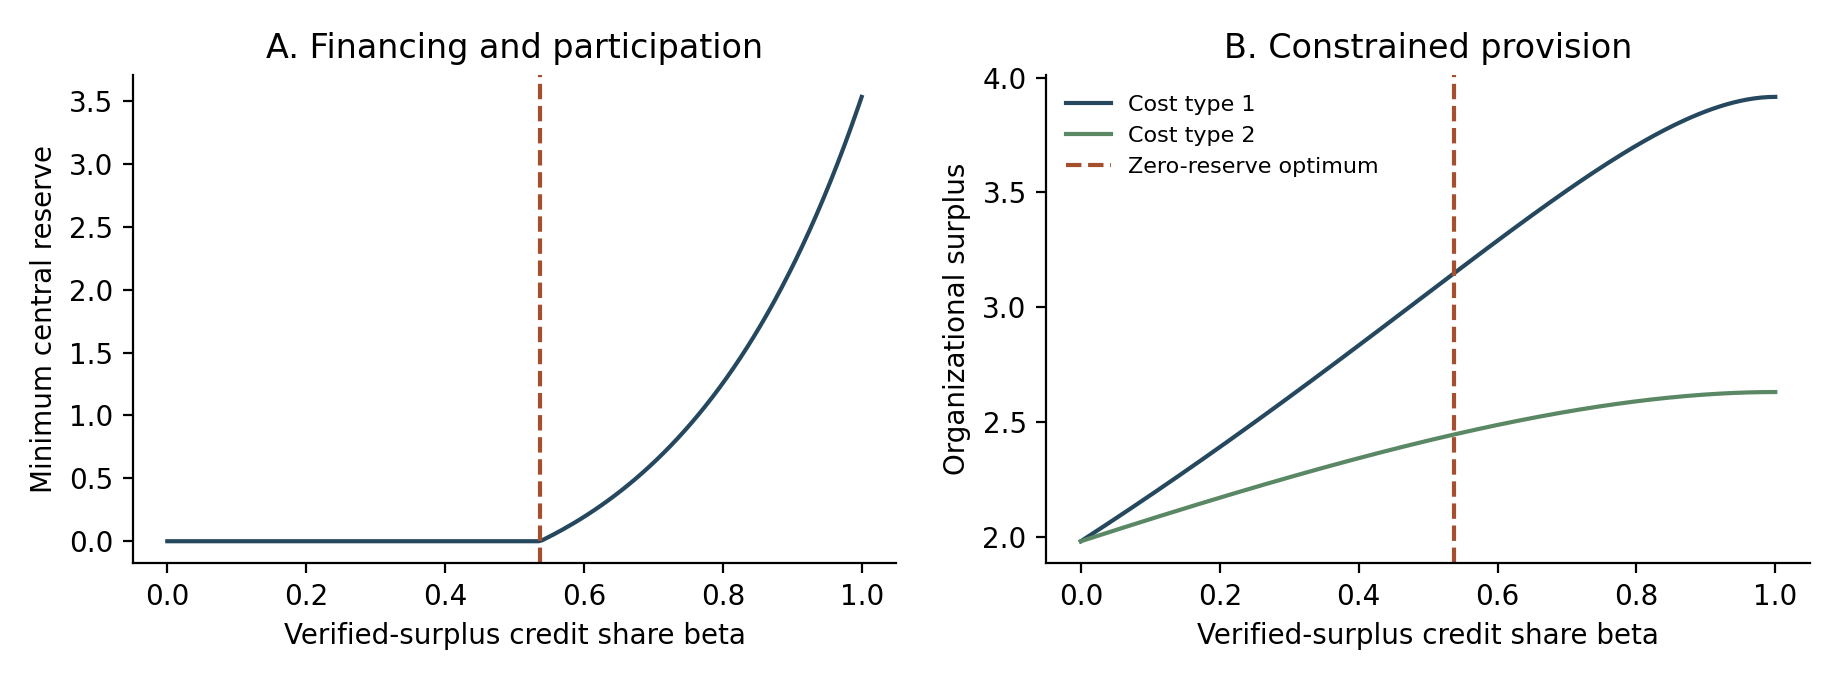
\includegraphics[width=0.95\textwidth,height=\textheight]{results_R1/financing.png}
\caption{Synthetic example: the zero-reserve frontier and surplus under
both private cost types. The dashed line marks the largest feasible
common credit share.}
\end{figure}

A separate binding-capacity solution uses the same primitives but
\(\bar L=2\). At \(\beta=1\), cost type 1 has
\((y_1,y_2)=(1.7867,.2133)\) and scarcity price \(\nu=.8808\); type 2
has \((1.6229,.3771)\) and \(\nu=.5330\). Both meet capacity exactly.
The model therefore includes genuine capacity rationing, rather than
substituting a convex-cost example for the hard constraint.

\subsection{8.3 Opposite interactions with two production
margins}\label{opposite-interactions-with-two-production-margins}

Use \(K=2I\), \(V=((1,.1),(.1,1))\), \(n=(1,1)\), \(a=(1,2)\),
\(\gamma=.1\), \(\bar L=100\), and \(\kappa=1\). Facilitation changes
\(h=(4,1)\) to \((4,2)\). Compare credit shares \(.4\) and \(.7\) under
the support-priced surplus score. All classes are interior and
\(\det V=.99\). The exact factorial differences are

\[\Delta q=-.0119774850,\qquad
\Delta d=.1679228408,\qquad
\Delta W=.1266561870. \tag{28}\]

Rational matrices and exact fractions in the reproduction output certify
the signs. This shows survival of the sign distinction as an allocation
example, not survival of the old scalar growth formula. The policies in
this example need not be financeable with \(B=0\); financing is
separately governed by (23).

\subsection{8.4 Verification actually
completed}\label{verification-actually-completed}

The active-set solver enumerates positive-use sets and capacity states.
An independent optimization of the original four-variable program checks
eight declared cases: interior use, excluded classes, no demand, zero
credit, and binding capacity. Maximum objective discrepancy was
\(2.87\times10^{-13}\) in the completed run. Exact rational calculations
isolate all financing-inequality roots in \([0,1]\) for Table 2 and
verify the largest feasible boundary, rather than assuming the reserve
function is monotone. Exact rational contrasts check (28). A strategic
gross-credit example independently verifies the strict welfare loss in
Proposition 4.

These calculations validate implementations of stated equations. The
proofs establish the results. Neither establishes empirical prevalence,
an effect size in euros, or the correctness of a firm-specific value
audit. The separately retained toy exposure estimator is not evidence
for the organizational mechanism and is not part of the theoretical
verification.

\subsection{8.5 Exact regression across the baseline
branch}\label{exact-regression-across-the-baseline-branch}

This single synthetic regression checks score levels and settlement, not
a parameter sweep. Set \(D=I\), \(a=(1,1)'\), \(K=2I\),
\(V=((1,1/5),(1/5,4/5))\), \(h=(4,-1/10)'\), \(\gamma=3/20\),
\(\bar L=10\), and \(\kappa=\beta=1\). Rational active-set enumeration,
separately implemented from the floating-point solver, gives

\[y_0=(80/23,0)',\qquad G(0)=160/23.\]

The first baseline KKT equation is \((23/20)y_{0,1}=4\), while the
excluded class has marginal gain \(-143/230<0\). The unconstrained
full-use baseline \(H^{-1}h=(71/20,-11/20)'\) is infeasible and has
quadratic value \(2851/400\). Hence

\[c_0=\frac{2851}{400}-\frac{160}{23}=\frac{1573}{9200}>0. \tag{29}\]

Solving \((H-VK^{-1}V')y=h\) and \(z=K^{-1}V'y\) independently gives

\[y=(5395/849,95/849)',\qquad z=(2707/849,385/566)'.\]

Both uses are positive, \(a'y=1830/283<10\), and \(\nu=0\). Condition
(A) and all investment/use KKT equalities are checked exactly. Strict
concavity therefore makes this the unique global surplus-score
allocation. At this allocation \(G(z)=33636065/1441602\). For the
incomplete R1 branch polynomial \(P=b'z+z'Jz/2\),

\[P-[G(z)-G(0)]=-1573/9200.\]

The exact ledger below evaluates the incomplete level at the same
allocation; it does not claim that the incomplete expression defines a
valid global scoring rule.

\begin{longtable}[]{@{}
  >{\raggedright\arraybackslash}p{(\columnwidth - 4\tabcolsep) * \real{0.3333}}
  >{\raggedleft\arraybackslash}p{(\columnwidth - 4\tabcolsep) * \real{0.3333}}
  >{\raggedleft\arraybackslash}p{(\columnwidth - 4\tabcolsep) * \real{0.3333}}@{}}
\toprule\noalign{}
\begin{minipage}[b]{\linewidth}\raggedright
Quantity
\end{minipage} & \begin{minipage}[b]{\linewidth}\raggedleft
Incomplete branch polynomial
\end{minipage} & \begin{minipage}[b]{\linewidth}\raggedleft
Actual constrained-baseline score
\end{minipage} \\
\midrule\noalign{}
\endhead
\bottomrule\noalign{}
\endlastfoot
Producer payment \(T\) & \(4672209349/288320400\) &
\(542973175/33156846\) \\
Rent \(r=T-C_\kappa\) & \(1893601/339600\) & \(448883/78108\) \\
Center deficit at fixed \(F=0\) & \(3768006349/288320400\) &
\(219494915/16578423\) \\
Maximum weak-IR fee, this single type & \(1893601/339600\) &
\(448883/78108\) \\
Reserve at that maximum fee & \(21603391/2883204\) &
\(21603391/2883204\) \\
\end{longtable}

Production cost is \(30645421/2883204\); support cost and
support-account surplus are both \(502335/160178\); support revenue is
\(502335/80089\). Actual payment is 16.3758994146, rent 5.7469529370,
and fixed-zero-fee deficit 13.2397945812. Each exceeds its incomplete
counterpart by \(c_0=.1709782609\). In this single-type ledger, raising
the maximal weak-IR fee by the same amount cancels the reserve
correction, giving 7.4928416442. At that fee participation is weak only.
Reducing the fee by \(\epsilon>0\) gives strict participation and raises
expenditure by \(\epsilon\).

In general, conditional on unchanged allocations, payment corrections
\(\Delta_\kappa\) change the reserve to

\[\left[m+\max_\kappa(T_\kappa+\Delta_\kappa-\Gamma_\kappa)
-\min_\kappa(r_\kappa+\Delta_\kappa)\right]_+. \tag{30}\]

At fixed common fee, each state's expenditure changes by
\(\Delta_\kappa\). A correction common to every type cancels from the
maximal-fee reserve; unequal corrections can change the fee-limiting and
deficit-generating types. Equal local derivatives alone guarantee
neither unchanged global branch choice nor unchanged financing. The
global score (14) is required.

Table 2 does not change: its baseline is \(y_0=(43/26,17/26)'\), with
both classes positive and slack capacity, so \(c_0=0\). R1's allocation
code already calculated the constrained \(G(0)\). Rerunning prior
examples and exact certificates reproduces \(\beta^*=.5370860743\),
\(F=.1627317858\), \(B_I(1)=3.5326121937\), and \(B_K(1)=2.2469100348\).
The regression compares the actual floating-point score, rent and
support ledger to the exact values and checks preserved R1 numerical
outputs. It rejects the incomplete score level even though a
derivative-only test would pass.

\section{9. Conclusion}\label{interpretation-and-limitations}

The allocation lesson is to separate the accounting units. Charge for
rival support and scarcity, and assess nonrival producer improvements
against verified incremental surplus. Using an average byte price to
recover all producer payments can distort heterogeneous admission.
Conversely, a technically correct support price can leave provision
underfunded. A common fee may recover rents without changing marginal
decisions, but voluntary participation caps how much it can raise.

The reserve constraint is a distribution and commitment constraint
inside an organization. It is not an additional social expenditure. A
draw from the reserve or a payment to the producer is a transfer; actual
investment effort, support, consumer implementation, and administration
are the resource costs. Scarcity rent is not counted as an extra benefit
in (4). The ledger can reconcile transfers without pretending that they
disappear from unit-level incentives.

The result does not select a data architecture or vendor. A central
authority with unrestricted consumer levies, fully verifiable producer
costs, or sophisticated screening may achieve a better frontier. A value
schedule that cannot be audited may make the proposed score unsuitable.
Private support coefficients, common risk constraints, support-capacity
investment, dynamic maintenance, and substitutes between source datasets
are omitted. The general network remains unsolved. Documentation raises
application value in this model; making it reduce support requirements
endogenously adds another nonseparable margin and is not covered by the
stated formulas.

The article establishes a joint allocation solution, a strategic scoring
distinction, and an exact reserve/participation frontier for a limited
accounting class. These are stronger results than the original
frozen-adoption cross-partials. They remain applications of familiar
incentive and club-good ingredients. The closest data-sharing comparator
is Rasouli and Jordan (2021), alongside public-goods financing and
internal transfer pricing. The restricted cross-type reserve calculation
does not exclude better mechanisms with quality distortion, consumer
assessments or richer contracts. The strongest rejection reason is that
the precise frontier may be judged too dependent on common-fee and audit
restrictions, and its empirical importance is unknown. The work is
complete at its theoretical scope; that does not establish publication
readiness or unrestricted originality.

A prospective field study is documented separately. It has no completed
observations and no implemented field-trial uncertainty pipeline. Its
need for partner authorization, auditable value measures, graph support,
and adequate independent clusters remains unchanged. None of those
future tasks is presented as an unfinished proof or a missing empirical
result in this theoretical article.


{
\small
\setlength{\parindent}{0pt}
\section*{References}\label{references}

Berglas, Eitan, and David Pines. 1981. ``Clubs, Local Public Goods and
Transportation Models: A Synthesis.'' \emph{Journal of Public Economics}
15(2): 141-162. \url{https://doi.org/10.1016/0047-2727(81)90030-X}.

Bierbrauer, Felix J. 2011. ``Incomplete Contracts and Excludable Public
Goods.'' \emph{Journal of Public Economics} 95(7-8): 553-569.
\url{https://doi.org/10.1016/j.jpubeco.2010.11.028}. Institutional working
version: \emph{An Incomplete Contracts Perspective on the Provision and
Pricing of Excludable Public Goods}, MPI 2010/01, revised April 2010.

Buchanan, James M. 1965. ``An Economic Theory of Clubs.''
\emph{Economica} 32(125): 1-14. \url{https://doi.org/10.2307/2552442}.

Cabrera, Angel, and Elizabeth F. Cabrera. 2002. ``Knowledge-Sharing
Dilemmas.'' \emph{Organization Studies} 23(5): 687-710.
\url{https://doi.org/10.1177/0170840602235001}.

d'Aspremont, Claude, Sudipto Bhattacharya, and Louis-Andre Gerard-Varet.
1998. ``Knowledge as a Public Good: Efficient Sharing and Incentives for
Development Effort.'' \emph{Journal of Mathematical Economics} 30(4):
389-404. \url{https://doi.org/10.1016/S0304-4068(97)00050-5}.

Dikolli, Shane S., and Igor Vaysman. 2006. ``Information Technology,
Organizational Design, and Transfer Pricing.'' \emph{Journal of
Accounting and Economics} 41(1-2): 201-234.
\url{https://doi.org/10.1016/j.jacceco.2005.06.001}.

Holmstrom, Bengt, and Paul Milgrom. 1991. ``Multitask Principal-Agent
Analyses: Incentive Contracts, Asset Ownership, and Job Design.''
\emph{Journal of Law, Economics, and Organization} 7, special issue:
24-52. \url{https://doi.org/10.1093/jleo/7.special}\_issue.24.

Jamm, Dominic. 2018. ``Intra-Organizational Knowledge Creation and
Sharing in a Principal-Agent Setting.'' \emph{FEMM Working Paper Series}
18001, Otto-von-Guericke University Magdeburg. Preliminary working
paper; later journal publication not verified.

Jones, Charles I., and Christopher Tonetti. 2020. ``Nonrivalry and the
Economics of Data.'' \emph{American Economic Review} 110(9): 2819-2858.
\url{https://doi.org/10.1257/aer.20191330}.

Rasouli, Mohammad, and Michael Jordan. 2021. ``Data Sharing Markets.''
\emph{arXiv} 2107.08630v2 {[}econ.TH{]}, 20 July 2021. Sections 4-5.
\url{https://arxiv.org/pdf/2107.08630v2}. Working paper; this comparison uses
that version.

Siemsen, Enno, Sridhar Balasubramanian, and Aleda V. Roth. 2007.
``Incentives That Induce Task-Related Effort, Helping, and Knowledge
Sharing in Workgroups.'' \emph{Management Science} 53(10): 1533-1550.
\url{https://doi.org/10.1287/mnsc.1070.0714}.

}
\clearpage
\section{Technical appendix: complete proofs and
boundaries}\label{technical-appendix-complete-proofs-and-boundaries}

\subsection{A. Existence, strict concavity, and the decentralized
equilibrium}\label{a.-existence-strict-concavity-and-the-decentralized-equilibrium}

Write \(\mathcal Y=\{y\geq0:a'y\leq\bar L\}\). It is nonempty and
compact since \(a_j>0\) and \(\bar L>0\). For the unpriced program use
the compact box \([0,\bar y]\). The block quadratic form for the
support-priced program (15) has negative Hessian with positive cost
matrix

\[\begin{pmatrix}\kappa K/\beta&-V'\\-V&H\end{pmatrix}. \tag{A1}\]

Its Schur complement is \(H-\beta Q/\kappa\succ0\) by (A). Thus it is
strictly positive definite for \(\beta\in(0,1]\), and the program is
strictly concave and coercive in \(z\). The same argument with \(H\)
replaced by \(D\) proves strict concavity of the joint unpriced
potential. Existence and uniqueness follow, including boundary optima.
At zero share, \(z=0\) is uniquely cost minimizing and strict concavity
in \(y\) gives a unique use allocation.

Maximizing first in \(y\) in the unpriced joint program produces (6),
after multiplication by \(\alpha\) and subtraction of the constant
\(\alpha G_D(0)\). This justifies the sequential comparison rather than
assuming a producer ignores induced demand. On an interior box branch,
the first-order conditions are \(Dy=h+Vz\) and \(\kappa Kz=\alpha V'y\).
Eliminating \(z\) gives (7). Substituting the identities into (4) gives
(8). Since \(M_D=D-\alpha Q/\kappa\) is symmetric positive definite and
\(dy/dh_j=M_D^{-1}e_j\), differentiating the quadratic expression (8)
yields (9). At entry or reservation boundaries use the unique
constrained program; the interior derivative is not extrapolated across
kinks. The constructed values in Table 1 directly verify a finite
harmful opening across an entry boundary.

\subsection{B. Full information, admission, and pricing
units}\label{b.-full-information-admission-and-pricing-units}

For the full-information program the positive definite block form is
(A1) at \(\beta=1\). Slater's condition holds for capacity using small
strictly positive eligible uses. The KKT conditions are necessary and
sufficient and give (10)-(11). The conditions for \(z\) are equalities
because \(K\) is diagonal and \(V'y\geq0\): whenever its component is
zero the associated investment is zero; otherwise the optimum is
positive.

At any fixed \(z\), a price-taking marginal user in class \(j\) requires
\(h_j+v_j'z-y_j/n_j-p_j=0\) when active and a weakly nonpositive
marginal gain at zero. Inserting (12) yields exactly the conditional
social KKT system. Strict concavity in \(y\) guarantees uniqueness. If
\(\ell<\bar L\) then \(\nu=0\). If \(\gamma=0\) and capacity is slack
then every required price is zero. With heterogeneous positive support
coefficients, two active classes and \(\lambda>0\), their required
application prices differ. An identical per-use price cannot satisfy
both necessary interior conditions. At corners or equal support
requirements the impossibility need not apply.

\subsection{C. Sequential scoring and the gross-credit
deviation}\label{c.-sequential-scoring-and-the-gross-credit-deviation}

The optimizer defining \(G\) is unique and lies in the compact set
\(\mathcal Y\). The envelope theorem gives \(\nabla G(z)=V'y(z)\),
including across a change in active class where the derivative remains
continuous. The producer's objective is
\(\beta[G(z)-G_0]-C_\kappa(z)-F\). It is equivalent to maximizing the
joint program multiplied by \(\beta\), because the outer maximum in
\(z\) commutes with the inner maximum in \(y\). Strict joint concavity
gives a unique producer and consumer allocation. This proves (15)-(16),
and using the \(y\)-KKT equations yields (17)-(18). A nonpositive
proposed scarcity multiplier or an invalid inactive-class inequality
means that proposed active set is discarded, not that a negative use is
permitted.

On a slack-capacity positive-use region, \(y(z)=H^{-1}(h+Vz)\) and
\(G(z)=\tfrac12(h+Vz)'H^{-1}(h+Vz)\). Subtracting the actual constrained
\(G_0=G(0)\) gives \(G(z)-G_0=c_0+b'z+z'Jz/2\), proving the level in
(19). If zero investment is on the same branch or its value-preserving
closure, \(G_0=\tfrac12h'H^{-1}h\) and \(c_0=0\). A baseline outside
that branch can give \(c_0\ne0\). Constants disappear only on
differentiation, not from transfers or participation. Each candidate in
(20) must obey its branch constraints; global comparisons use the
constrained value function. The gross score is
\(\beta z'V'H^{-1}(h+Vz)\), which has twice the quadratic term.
Differentiating gives (20). With \(\beta=1\), the correct optimum is the
unique welfare optimum. If \(Jz_F\ne0\), evaluating the gross
first-order condition there leaves a nonzero derivative, so the gross
optimum differs; strict concavity of true welfare makes its welfare
strictly smaller. The proposition is conditional on the gross
objective's stated positive definiteness and interior uses; it makes no
claim of a finite optimum otherwise.

\subsection{D. Reserve theorem, private costs, and
participation}\label{d.-reserve-theorem-private-costs-and-participation}

Once the type-specific allocation is chosen, the producer's net
incremental payoff is \(r_\kappa-F\). Ex-post voluntary participation
for every type requires \(F\leq\min_\kappa r_\kappa\). Since \(z=0\) is
available before the fee is paid, optimized rent is nonnegative.
Conditional on acceptance, \(F\) is constant in investment and does not
change its maximizer. The center's net expenditure is

\[T_\kappa+S(\ell_\kappa)+m-\lambda_\kappa\ell_\kappa-F
=T_\kappa-\Gamma_\kappa+m-F. \tag{A2}\]

Requiring (A2) to be at most \(B\) for every type gives the lower bound
in (24). Combining it with participation and \(F\geq0\) proves necessity
and sufficiency of (23). Taking the largest participating fee minimizes
the needed reserve. No cost type is reported in implementing that common
fee.

If type is verifiable, choose \(F_\kappa=r_\kappa\), giving zero
incremental producer rent and expenditure \(c_\kappa-\Gamma_\kappa+m\).
This proves (25). For each type, \(r_\kappa\geq\min r\), so
\(T_\kappa-\Gamma_\kappa-\min r\geq c_\kappa-\Gamma_\kappa\). Maximizing
and taking the positive part establishes \(B_I\geq B_K\). The inequality
is strict in Table 2, so it is not an algebraic equality disguised as an
informational constraint.

This proof establishes only what the designated fee and credit family
can implement. A fee conditioned on output, a menu, or fixed consumer
assessments can change both constraints. Private costs alone do not
logically prohibit such mechanisms. With strict participation and a
binding bound, the upper bound becomes open as stated in Section 6.

\subsection{E. Monotonic welfare, existence of the constrained optimum,
and audit
error}\label{e.-monotonic-welfare-existence-of-the-constrained-optimum-and-audit-error}

Let \(g_i=G(z_{\beta_i})-G_0\) and \(c_i=C_\kappa(z_{\beta_i})\) for
\(0\leq\beta_1<\beta_2\leq1\). Producer optimality at both shares gives

\[\beta_1(g_2-g_1)\leq c_2-c_1\leq\beta_2(g_2-g_1). \tag{A3}\]

Adding the optimality inequalities first yields \(g_2\geq g_1\).
Consequently true-surplus change is
\(g_2-g_1-(c_2-c_1)\geq(1-\beta_2)(g_2-g_1)\geq0\). This argument covers
entry, exit, binding capacity, and zero credit without
differentiability. Constant \(m\) does not change the ordering.

Allocations and the value function are continuous in \(\beta\) on
\([0,1]\) under strict concavity and compact/coercive feasibility. The
support multiplier is unique whenever capacity binds with positive load:
an active positive class identifies it; at transitions it matches the
slack value zero. At no demand choose \(\nu=0\). Thus \(r,T,\Gamma\),
and \(B_I\) are continuous in this model, and the feasible share set is
closed in a compact interval. A nonempty set has a largest element.
Applying (A3) separately to every type proves Theorem 2 for arbitrary
type probabilities, without assuming the budget function is monotone. A
fixed administration cost may leave the feasible set empty; the theorem
explicitly conditions on nonemptiness.

On a smooth active branch differentiate \(\beta\nabla G=\kappa Kz\) to
obtain (27). \(\kappa K-\beta G_{zz}\) is positive definite by strict
concavity of the reduced problem. The gradient relation shows
\(\kappa z'Kz_\beta\geq0\). For a factor-inflated score, replacing
\(\beta\) by \(\widetilde\beta\) proves the audit-error statement
whenever the effective share is at most one. Budget feasibility requires
a separate worst-case calculation for actual payments. There is no claim
that a failed audit bound still implements the frontier.

\subsection{F. Preserved scalar benchmark and its restricted
interpretation}\label{f.-preserved-scalar-benchmark-and-its-restricted-interpretation}

For fixed downstream adoption, let gross reusable value per module be
\(B(t)\geq0\), linear producer cost \(D_0(t)\), quadratic cost curvature
\(K_c(t)>0\), and private appropriation \(\alpha\). Then
\(q_D=[\alpha B-D_0]_+/K_c\) and constrained optimum
\(q_C=[B-D_0]_+/K_c\). When \(B>D_0\), completing the square gives
welfare loss \(K_c(q_C-q_D)^2/2\). On an interior branch,

\[q_{D,\alpha}=B/K_c,\quad
\widetilde W_\alpha=(1-\alpha)B^2/K_c. \tag{A4}\]

Differentiating in \(t\) gives quantity complementarity if
\(B'/B>K_c'/K_c\), and surplus complementarity if \(2B'/B>K_c'/K_c\),
for \(\alpha<1\). For general scalar convex costs replace \(K_c\) by
cost curvature evaluated along the equilibrium branch; that curvature
itself then depends on the allocation. This is the former result, fully
conditional on a scalar investment object. It is not used to prove
Theorems 1-2 or to infer the multi-margin signs in (28).

\subsection{G. Reproduction and accounting
boundaries}\label{g.-reproduction-and-accounting-boundaries}

The active-set algorithm checks all positive-use subsets, then slack or
binding capacity, using (17)-(18). For the unpriced comparison it checks
lower/free/upper reservation states. It enforces inactive inequalities,
positivity, and the physical limit. Independent constrained optimization
uses the unreduced objective, rather than reusing the reduced
first-order conditions. The exact financing certificate rewrites each
requirement \(T_\kappa-\Gamma_\kappa-r_{\kappa'}\leq0\) as a rational
polynomial inequality for the declared zero-reserve example, isolates
all roots, and checks intervals. It is a certificate for the example,
not a universal assertion that feasible shares form an interval.

No synthetic dataset is labeled as observed. Copies of external papers
are not redistributed. The archive includes the original assignment,
central reviews, editable sources, executable code, output tables and
figure, reference audit, and numbered revision responses. The current
entry point is \texttt{python3\ code/reproduce\_R2.py}; it reruns R1 and
the exact crossing-baseline score and settlement regression in Section
8.5. The regression also verifies that the preserved numerical R1 files
are byte-identical after rerunning. The historical field protocol is
clearly prospective and cannot validate this mechanism until an
authorized study is executed.

\end{document}
